\documentclass{article}
\usepackage{amsthm}
\usepackage{amsmath}
\usepackage{graphicx}
\usepackage{subfigure}
\usepackage{verbatim}
\usepackage{glossaries}
\newtheorem{theorem}{Theorem}[section]
\newtheorem{corollary}[theorem]{Corollary}
\newtheorem{defination}{Definition}[section]
\begin{document}
\section{Approach}
In this article, we name the MAC scheme adopted in Cost-Effective Tag Design\cite{} CETD-MAC. 
\subsection{Specification of the MAC Scheme in Cost-Effective Tag Design}
In this section, we depict the design details of CETD-MAC scheme. At the beginning we express notations required to understand CETD-MAC scheme. 

\paragraph{Notations}
Let \{0,1\}$^n$ be the set of all n-bit binary strings. The set of all binary string is expressed as \{0,1\}$^*$.  
For a string X $\in$ \{0,1\}$^n$, |X| is its length in bits, and $\vert$ X $\vert$ $_l$ = $\lceil$$\vert$ X $\vert$/l$\rceil$ is the length of X in l-bit blocks.  Let 0$^l$ and 1$^l$ denote bit strings of all zeros and all ones. 
For a bit string X and an integer l that $\vert$ X $\vert$ $\geq$ l, msb$_l$(X) denotes the most significant l bits(left most l bits) of X and lsb$_l$(X) for least significant l bits(right most l bits) of X.
For two bit string X and Y, we denote X$\|$Y  or XY as the their concatenation. For bit string X whose length in bits is multiple of integer l, we denote X parted into l-bit sub-strings as X = (X[1]X[2]$\ldots$X[n])$_l$, where X[1], X[2], $\ldots$, X[n] $\in$ \{0,1\}$^l$.
The number of bits in a string of X is denoted as len(X).

The block cipher encryption of a string X with a secret key K is denoted as E$_K$(X). E$_K$(X) expresses the String mapping of \{0,1\}$^n$ $\rightarrow$ \{0,1\}$^n$ where n is the len(X) and len(output).
\paragraph{CETD-MAC Scheme}
CETD-MAC scheme can be expressed as tag = CETD-MAC(M, nonce-input). The input arguments of CETD-MAC are message M and a tuple named nonce-input. The tuple nonce-input is the concatenation of the memory address of M, a counter and a random number, denoted as nonce-input=(address$\|$counter$\|$random). The length of nonce-input, len(nonce-input), is identical to the length of input to block cipher E$_K$(X). The output of CETD-MAC is named tag, whose length is optional. We use Sub-BLK-No to express the value of  len(M)/len(tag). One prelimary of CETD-MAC is that Sub-BLK-No should be no less than 2 to assure that swapping stage can work and 0s will be concatenated to the leftmost of input message when Sub-BLK-No is not integer.  

We follow the defination of CETD-MAC in \cite{keylist}. 
\begin{itemize}
	\item Message is splitted to sub-blocks each of whose length is tag length
	\item The first stage is several rounds of bit-segment swapping. For each round , two sub-blocks are randomly chosen. Introduce shuffle paremeter V[i]
	\item The output sub-blocks from swapping stage, named X blocks, are sent to block-level rotate shifting stage. Each X block is rotate shifted for several bits. Introduce shift parameter S[i]
	\item The output sub-blocks from shifting stage, named Y blocks, are XORed to form the final tag
\end{itemize}
\paragraph{The Identity of Sets}
Assume there are two sets, marked as X\_A and X\_B, having same NO. of elements and the number is M. Each element is given an index from 1 to M. The definition of Identical Index Equality is expressed here:
\begin{defination}
Identical Index Equality(IIE): For any i$\in$[1,M], X\_A[i]=X\_B[i].
\end{defination}
The definition of Cross Index Equality is expressed here:
\begin{defination}
Cross Index Equality(CIE): For any i,j$\in$[1,M], X\_A[i] = X\_B[j], where i$\neq$j
\end{defination}

Any two sets that have same number of elements can be splited into several sub-groups and each sub-groups contains several (X\_A[i],X\_B[i]) pairs. For two specific sets, the number of sub-groups various from 1 to M. We give the definition of set level equality of two sets with same number of elements:
\begin{defination}
Set Level Equality(SLE): Each sub-group have one of the two kinds of Equality.
\end{defination}

For two sets X\_A and X\_B, if there is no way of spliting that at least one sub-group is of CIE and there are at least one way of split that all sub-sets are of IIE, then such X\_A and X\_B are IIE only Sets. 
The definition of CIE only Sets is given in same way.


\subsection{Tag Collision Under Replay Attack}
In this section, we depicit the weaknesses we found in CETD-MAC under replay attack. These weaknesses in mechanism let the CETD-MAC to produce tags with high collision probability with some chosen inputs. The tags with highly collision probability ease the adversary`s attack.
\paragraph{Security Notion of MAC Schemes under Replay Attacks}
We adopt the standard notion for the security of a MAC scheme in the presence of a replay attack, in which an adversary is given  access to a tag generation black-box(named oracle) and a message-tag pair verification oracle. The encryption key is maintained unchanged while the nonce value is updated for each calling of tag generation oracle no matter whether the value of input message collide with a value in old timestamp. The adversary can record the message-tag pairs in old time stamp to copies and replace a pair in new timestamp with a piece of copies. The forgery advantage F$_{CETD-MAC}$ under replay attack is the probability that the adversary can get the verification oracle to accept a copy with old timestamp at a new time point. 

Assume the copy with old timestamp from the adversary is expressed as (M1,T1) where M1 is the messsage and T1 is the corresponding tag, and the correspoding nonce is denoted as N1. When applying M1 to the tag generation at a new time point, we mark the corresponding tag T2 and nonce N2. If the adversary can succeed a replay attack, then T1 is identical to T2.
Then F$_{CETD-MAC}$ under replay attack can be denoted as a probability Pr[T1 = T2  $\mid$ Message value is M1 \& N1,N2 are randomly generated]. 

\paragraph{Tag Collision Expressed with Y blocks}
According to the design of CETD-MAC, the tag can be expressed as Y[1]$\oplus$Y[2]$\oplus$$\ldots$$\oplus$Y[x], x is the number of input sub-blocks to CETD-MAC. If two tags T1 and T2 are identical, the following equation is met:
Y$_1$[1]$\oplus$Y$_1$[2]$\ldots$$\oplus$Y$_1$[x]$\oplus$Y$_2$[1]$\oplus$Y$_2$[2]$\ldots$$\oplus$Y$_2$[x] = 0, where Y$_1$ blocks produce T1 and Y$_2$ blocks generate T2.
\subsubsection{The Block-level Pattern Collision}
As the nonce is generated by block cipher encryption E$_K$. Assume E$_K$ performace like a ideal random value generator, for two distinct input nonce-input1 and nonce-input2, the corresponding nonce values N1 and N2 should be random and the probability that N1 is identical to N2 should be 1/2$^n$, where n is len(N1). 
We regard blocks from a operation stage in CETD-MAC as a sequence and each block has a distinct index i$\in$[1,x] where x is the number of blocks. 
In this section, we express the first weakness in the rotate shifting stage in CETD-MAC. 
\begin{defination}
If the a input block of rotate shifting stage X$_1$[i ]from X1 sequence is identical to the block X$_2$[i] with same index from X2 sequence, the following two properties exist:
\begin{itemize}
	\item The probability that correspoding output blocks of rotate shifting stage, Y$_1$[i] and Y$_2$[i], are identical can be expressed with the length of pattern in X$_1$[i].	
	\item The more identical X block pairs(X$_1$[i],X$_2[i]$) are formed by repeating pattern, the higher probability of identical block pairs in Y sequences (Y$_1$[i],Y$_2[i]$) exist, then the higher probability of tag collision(T1=T2)
\end{itemize}
\end{defination}
These two properties measn if the adversary conduct replay attack on the memory frame whose message part is formed with pattern, then the probability of successful forgery, expressed as F$_{CETC-MAC}$, is high.

If the elements in identical sub-sets of two X sets are formed by pattern, then the corresponding two Y sub-sets, Y$_{sub}$1 and Y$_{sub}$2, have high probability to be IIE.

\subsubsection{The Set-level Pattern Collision}


If any element in identical sub-sets of two X sets can be formed by rotate shifting another element in the same sub-set, the corresponding two Y sub-sets, Y$_{sub}$1 and Y$_{sub}$2, have high probability to be SIE.

\subsection{A Solution to Elimitated the Collision}
In this section we provide an modification of original CETD-MAC. Our approach does not require additional component or information to the original CETD-MAC. We then prove that the optimized CETD-MAC can fix the weakness and protect input message from replay attack.

\section{The Collision Probability of Y Set}

\subsection{Preliminaries}
\paragraph{The Equality of Two Sets}
Assume there are two sets, marked as X\_A and X\_B, having same NO. of elements and the number is M. Each element is given an index from 1 to M. The definition of Identical Index Equality is expressed here:
\begin{defination}
Identical Index Equality(IIE): For any i$\in$[1,M], X\_A[i]=X\_B[i].
\end{defination}
The definition of Cross Index Equality is expressed here:
\begin{defination}
Cross Index Equality(CIE): For any i,j$\in$[1,M], X\_A[i] = X\_B[j], where i$\neq$j
\end{defination}

Any two sets that have same number of elements can be splited into several sub-groups and each sub-groups contains several (X\_A[i],X\_B[i]) pairs. For two specific sets, the number of sub-groups various from 1 to M. We give the definition of set level equality of two sets with same number of elements:
\begin{defination}
Set Level Equality(SLE): Each sub-group have one of the two kinds of Equality.
\end{defination}

For two sets X\_A and X\_B, if there is no way of spliting that at least one sub-group is of CIE and there are at least one way of split that all sub-sets are of IIE, then such X\_A and X\_B are IIE only Sets. 
The definition of CIE only Sets is given in same way.

\subsubsection{Replay Attack and Y Set Collision}
\paragraph{The Message Sets in CETD Under Replay Attack}
The Cost-Effective Tag Design can be expressed as the following procedure:
\begin{itemize}
	\item The data is split into blocks. The block length is tag length. The block set is marked as D, and the No. of blocks is M.
	\item The content of blocks are shuffled. The output set of shuffle is marked as X.
	\item The content of each block is rotate shifted. The output set of rotate shift is marked as Y.
	\item All the blocks in Y is XORed to form the tag T.
	\item The control parameters is retrived from the segment of nonce N. The parameter set of shuffle is marked as S. The set for rotate shift is R.
\end{itemize}

In replay attack, the adversary replaces a data-tag pair on the memory with a
pair copied from the same address at an old time point. That means for the two
pairs at different time point, the two message block sets D\_A and D\_B and related tags T$_a$ and T$_b$ are
identical respectively, while the nonce N$_A$ and N$_B$ are randomly generated and
the equality is unpredictable if their generator is of high quality. The shifting bits parameter segment on the nonce R\_A and R\_B, are randomly
generated.
We can see that if the Y set for the old time point, marked as Y\_A, is SLE to the Y set for new time point, marked as Y\_B, T$_a$=T$_b$.
Based on the concept of set equality, the message block sets in the generation of T$_a$ and verification of T$_b$ meet the following properties if the replay attack succeeds:
\begin{itemize}
	\item D\_A and D\_B are IIE.
	\item If the shuffle stage does not work. X\_A=D\_A, X\_B=D\_B
	\item Y\_A and Y\_B are SLE
\end{itemize}

In this scenario, the probability of a successful attack can be expressed as the equation 1.1:
\begin{defination}
Pr[Successful Replay Attack] = Pr[T$_a$ = T$_b$ $\mid$ (D\_A = D\_B) \& (R\_A and R\_B are random)]
							 = Pr[Y\_A = Y\_B $\mid$ (D\_A = D\_B) \& (R\_A and R\_B are random)]
							 
D\_A and D\_B sets are of Identical Index Equality. Y\_A and Y\_B is of Set Level Equality.
\end{defination} 
For easy understanding, we assume the shuffle stage does not work at first, which means D\_A = X\_A = D\_B = X\_B(IIE). Hence the Y set is the output of rotate shifting stage in CETD, we will analyze the properties of block rotate shifting and the cases of input sets that can result Y set collision(SLE). 

\begin{figure}[htbp]
 \centering
 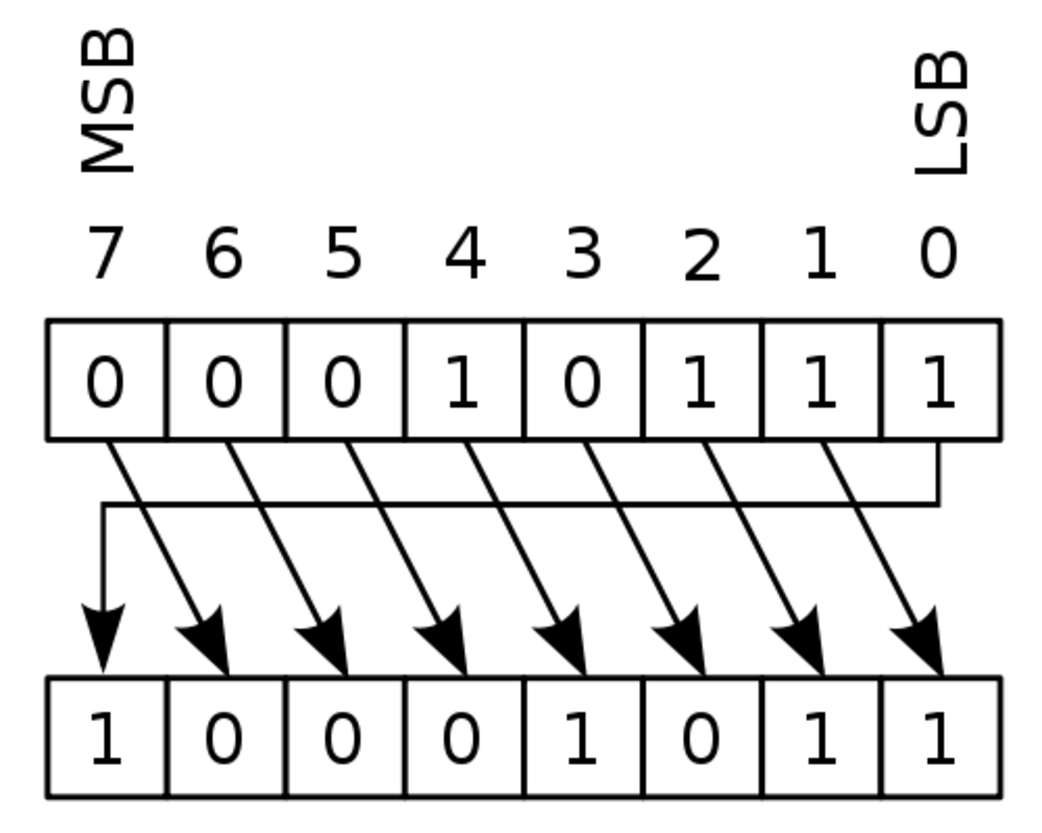
\includegraphics[scale=0.4]{./diagrams/rotate_right.pdf}
 \caption{The Concept of Rotate Shifting(Right)}
 \label{fig:1 }
\end{figure}

\subsubsection{Rotate Shifting Introduction} 
Unlike logical shifting and arithmetic shifting, rotate shifting
behaves like whirling a wheel. The empty position in a message block shifted is
filled by the bits shifted out. Figure 1 express the concept of rotate shift.

We can refer that the result of rotate shifting a message block depends on the
value of block and the bits shifted.  If two message blocks whose value are
identical are shifted with distinct bits, the result blocks may be
identical. That means when shifting bits fixed,the mapping from X blocks to the
shifted result blocks is not injection. This case is expressed in Figure 2(a).

For two distinct X blocks, however, their result blocks may be identical
when their shifting bits are distinct. This case is expressed in Figure 2(b).  
When the shifting bits of two message blocks are identical, the equality of result blocks
is same as the equality of their input blocks.				

\begin{figure}
\centering
\subfigure[Same Block Shifted Different Bits]{
\begin{minipage}[b]{0.45\textwidth}
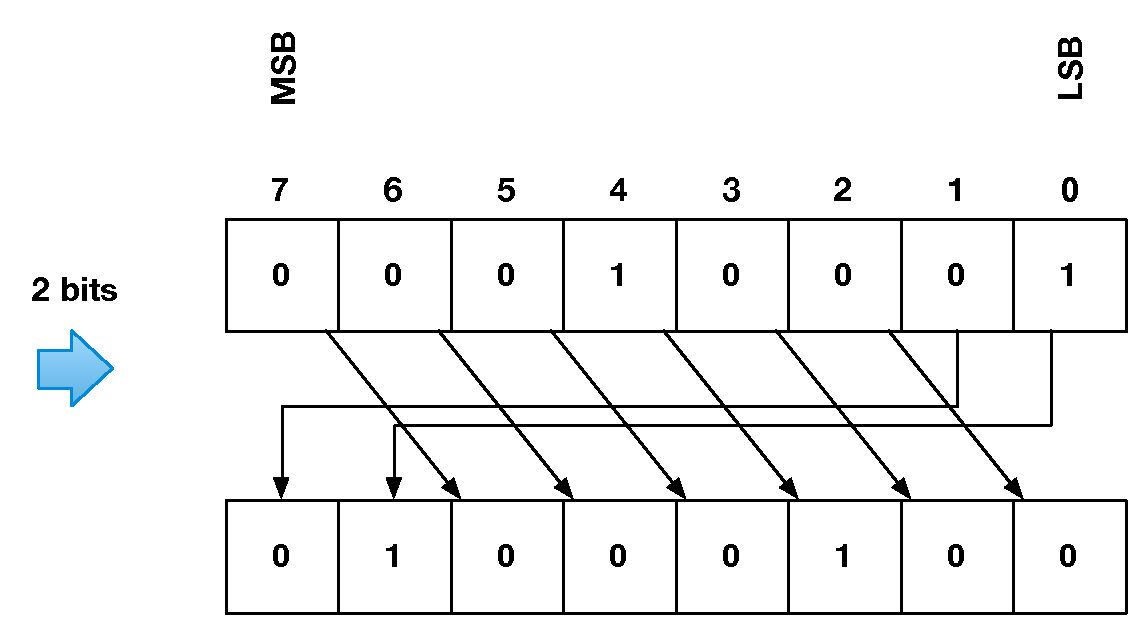
\includegraphics[width=1\textwidth]{./diagrams/r_s_2bits.pdf} \\
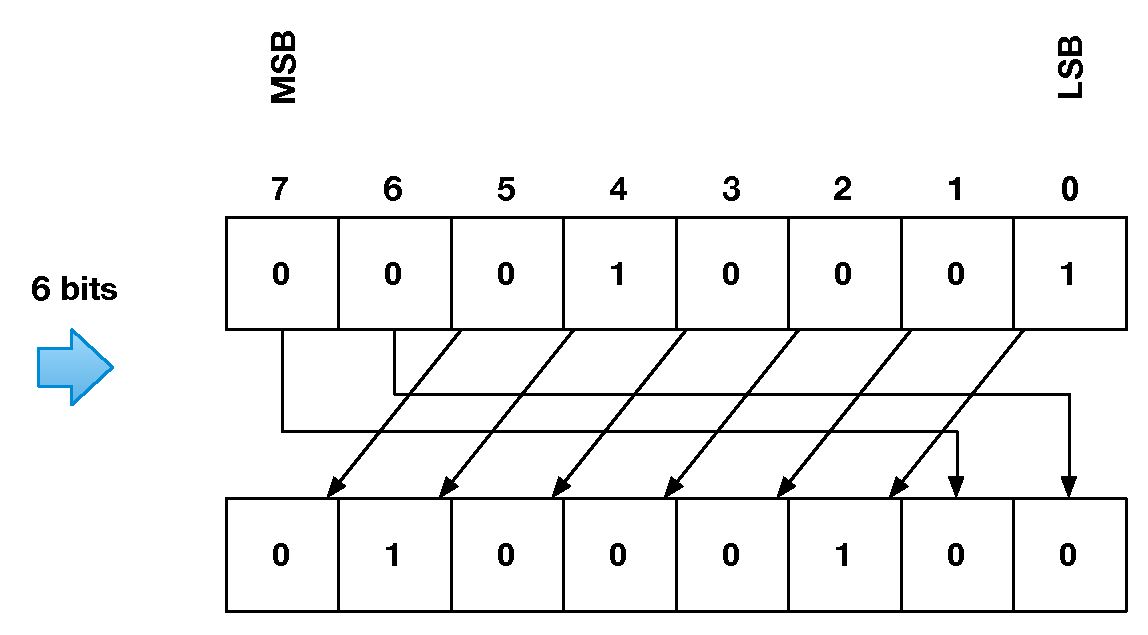
\includegraphics[width=1\textwidth]{./diagrams/r_s_6bits.pdf}
\end{minipage}
}
\subfigure[Different Blocks Shifted Different Bits]{
\begin{minipage}[b]{0.45\textwidth}
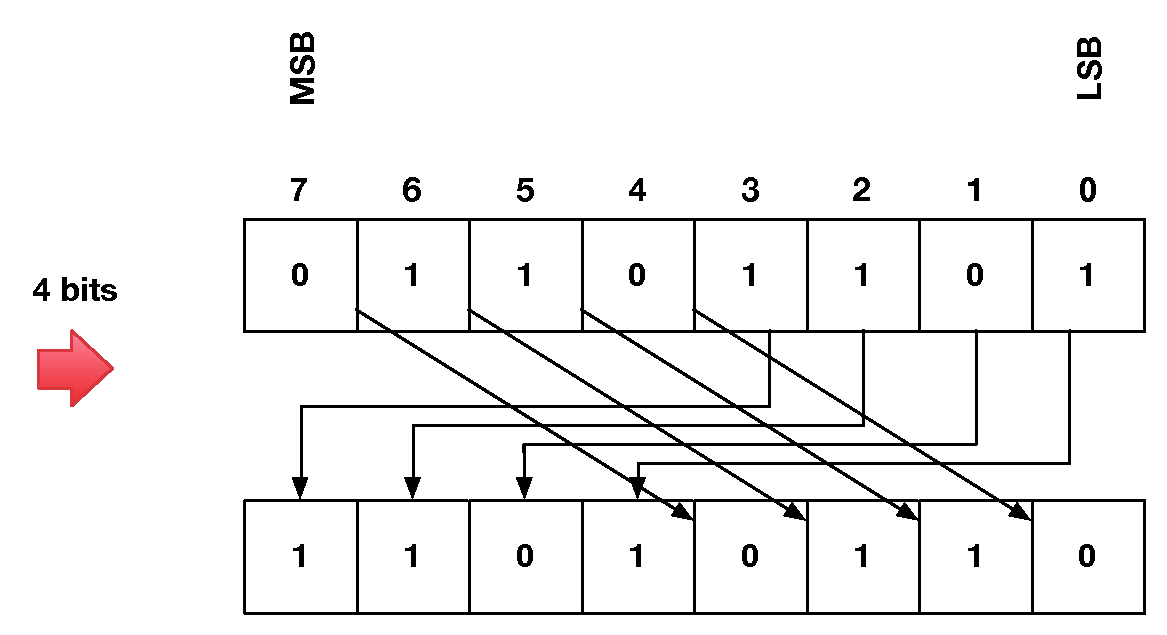
\includegraphics[width=1\textwidth]{./diagrams/r_d_4bits.pdf} \\
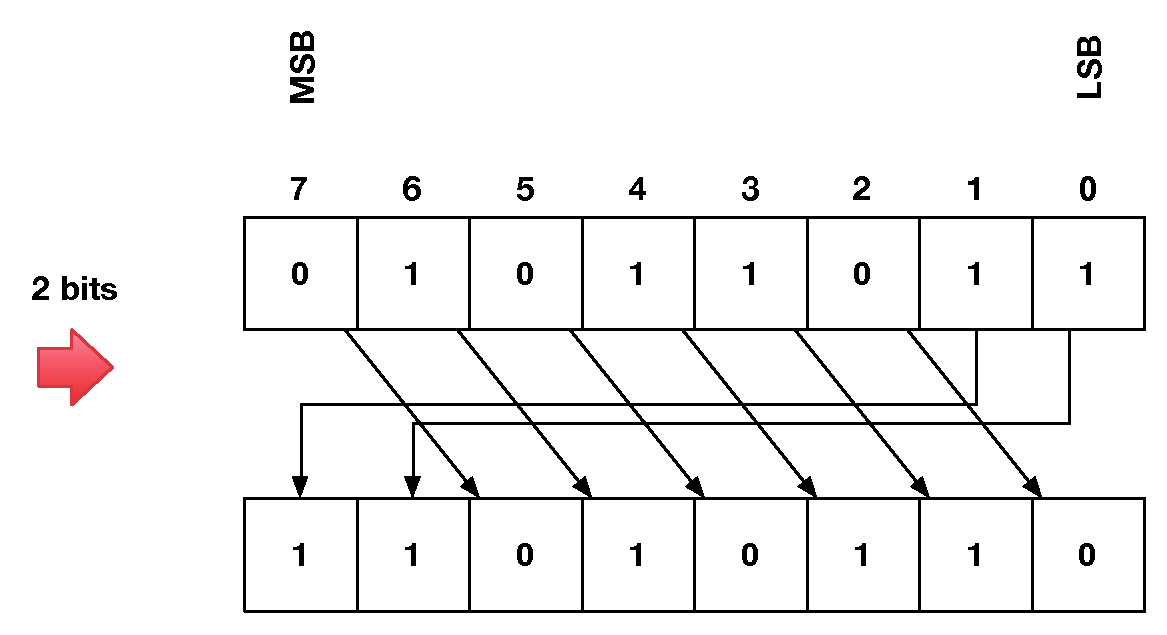
\includegraphics[width=1\textwidth]{./diagrams/r_d_2bits.pdf}
\end{minipage}
}
 \caption{The Examples of Y Block Collision}
 \label{fig:2 }
\end{figure}


\begin{figure}
\centering
\subfigure[Only Single Block Equality]{
 \label{fig:y_single_e} %% label for first subfigure
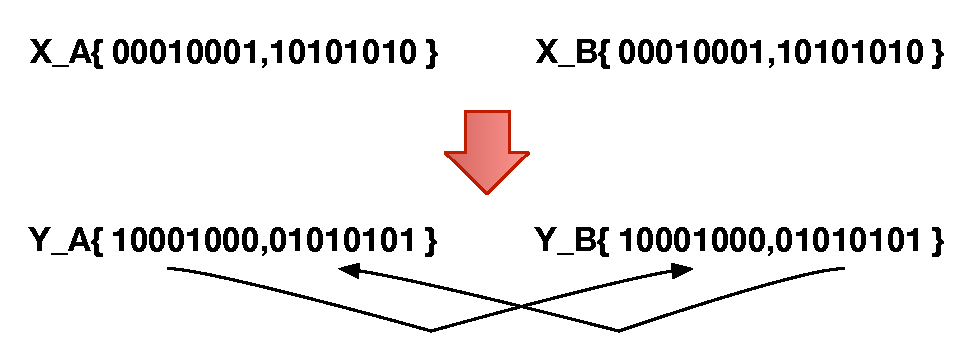
\includegraphics[width=.5\textwidth]{./diagrams/y_single_equality.pdf}
}
%\hspace{1in}
\subfigure[Only Set Level Equality]{
\label{fig:y_set_e} %% label for second subfigure
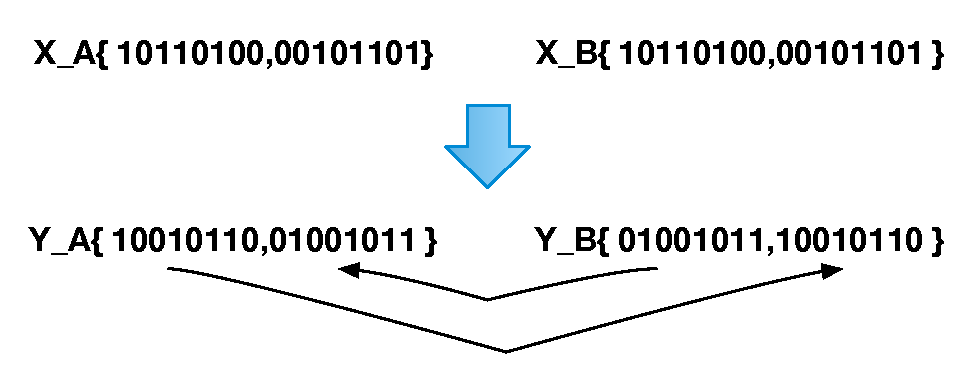
\includegraphics[width=.5\textwidth]{./diagrams/y_set_equality.pdf}
}
\caption{X Set Pairs with Only One Type of Y Equality}
 \label{fig:y_e_single} %% label for entire figure
\end{figure}

\begin{figure}
\centering
\subfigure[Single Block Equality Case]{
 \label{fig:y_both_single} %% label for first subfigure
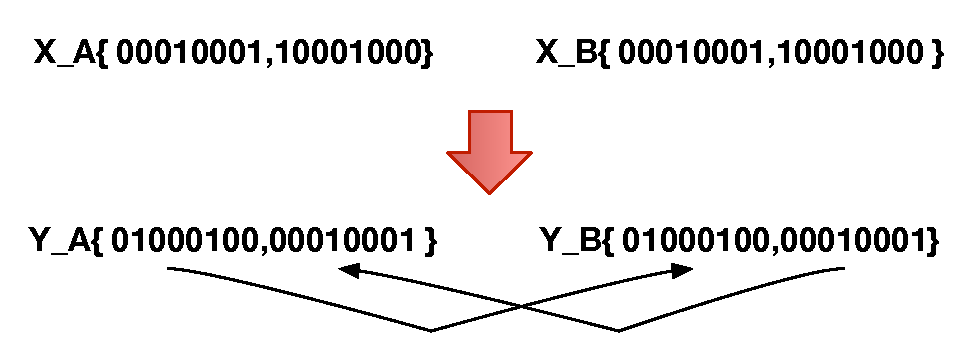
\includegraphics[width=.5\textwidth]{./diagrams/y_both_single.pdf}
}
%\hspace{1in}
\subfigure[Set Level Equality Case]{
\label{fig:y_both_set} %% label for second subfigure
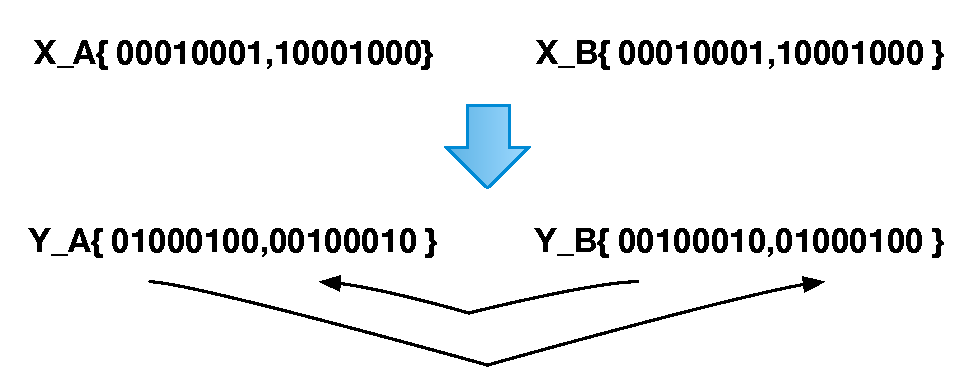
\includegraphics[width=.5\textwidth]{./diagrams/y_both_set.pdf}
}
\caption{A X Set Pair with Two Types of Y Equality}
 \label{fig:y_both} %% label for entire figure
\end{figure}

\subsection{Rotate Shifting and Y Set Collision} 
Assume the shuffle stage does not work, then D\_A= X\_A=D\_B=X\_B, which means the following properties exist in X\_A and X\_B:
\begin{itemize}
	\item X\_A[i] = X\_B[i] for all i$\in$[1,M], M is the number of elements
	\item The equality of elements in a X set is uncertain.
\end{itemize}
Then X\_A and X\_B are of Identical Index Equality. 
All the analysis in this section is based on the assumption that shuffle stage does not work.

If such X\_A and X\_B result two Y sets of Set Level Equality, the related tag T$_a$ = T$_b$.
 
Figure 3 and Figure 4 express the examples of X sets that lead to SLE Y sets with distinct R sets. In this paper, we analyze the cases of the input set pair (X\_A and X\_B) of shifting stage in CETD under replay attack that can lead to Y set pair collision(SLE).



\subsubsection{Case of X Sets Resulting Y Set Collision}
If R\_A and R\_B are IIE, then for any two identical set X\_A and X\_B, Y\_A and Y\_B are IIE. If there is at least one pair of blocks in R\_A and R\_B, marked as (R\_A[i], R\_B[i]), is distinct, then equality of Y\_A and Y\_B is uncertain.

Assume the number of distinct block pairs in R\_A and R\_B is R$_d$. For these R block pairs, their related X\_A and X\_B blocks formed a sub-group, marked as X\_A$_s$ and X\_B$_s$, and this sub-group is IIE. The related sub-group in Y\_A is marked as Y\_A$_s$ and the one in Y\_B for Y\_B$_s$.

In this part, we discuss the equality case of Y\_A$_s$ and Y\_B$_s$
\paragraph{Identical Index Equality Case}
If Y\_A$_s$ and Y\_B$_s$ are IIE, then for all i$\in$[1, R$_d$] the following two properties are met:
\begin{itemize}
	\item Y\_A$_s$[i] = Y\_B$_s$[i] 
	\item R\_A$_s$[i] $\neq$ Y\_B$_s$[i]
	\item X\_A$_s$[i] = X\_B$_s$[i]
\end{itemize}
Figure 2(a) provides a instance of IIE Y sets.
The identical block pairs (X\_A$_s$[i],X\_B$_s$[i]) that lead to IIE Y\_A$_s$ and Y\_B$_s$ have the property in Theorem 1.1:
\begin{theorem}
Assume X\_A[i] and X\_B[i] are two identical block from two sub-group X\_A$_s$ and X\_B$_s$ with same index i. X\_A[i] and X\_B[i] have same number of bits N=2$^n$. The result of rotate shifting X\_A[i] and X\_B[i] with distinct shifting bit parameter R\_A[i] and R\_B[i] are marked as Y\_A[i] and Y\_B[i]. 

Then Y\_A[i] and Y\_B[i] can be identical only when X\_A[i] and X\_B[i] are formed by repeating a binary pattern P, which is a binary segment. The length of this pattern P can be expressed as:

	P\_L = 2$^p$, p$\in$[0,n-1]
\end{theorem}
Base on Theorem 1.1, we got the following corollaries:
\begin{corollary}
If a pattern is not formed by a pattern with short length, we call it a distinct pattern of length P\_L. The No. of distinct patterns with length P\_L= 2$^p$ is 2$^{2^p}$-2$^{2^{p-1}}$
\end{corollary}
\begin{corollary}
Assume the length of a block is N=2$^n$, then the No. of all distinct patterns with all possible length is 2$^{N/2}$
\end{corollary}

\paragraph{Cross Index Equality Case}
If Y\_A$_s$ and Y\_B$_s$ are CIE, then for all distinct (i,j) that i,j$\in$[1, R$_d$] the following two properties are met:
\begin{itemize}
	\item Y\_A$_s$[i] = Y\_B$_s$[j] 
	\item R\_A$_s$[i] $\neq$ Y\_B$_s$[i]
	\item X\_A$_s$[i] = X\_B$_s$[i]
\end{itemize}
Figure 2(b) provides an instance of CIE Y sets.
The blocks in X\_A$_s$ and X\_B$_s$ that lead to CIE Y\_A$_s$ and Y\_B$_s$ have the property in Theorem 1.2:
\begin{theorem}
If Y\_A$_s$ and Y\_B$_s$ are CIE, each element in X\_A$_s$ can be formed by rotate shifting another element in X\_A$_s$.
\end{theorem}

If each element in X\_A$_s$ is formed by a pattern can be formed by rotate shifting another element in X\_B$_s$ then the related Y\_A$_s$ and Y\_B$_s$ can be either IIE or CIE or SLE.
The proof of Theorem 1.1 and Theorem 1.2 can be refered in appendix.


\subsection{The Probability of Y Set Collision} 
Hence the shift bit parameter set R\_A and R\_B are randomly generated, the probability of Y set collision for each input case is determined by the number of specific combinations of R\_A and R\_B. The computation of Pr[Y\_A = Y\_B] is based on this idea.
The following properties are met by any cases of D sets and R sets in replay attack:
\begin{itemize}
	\item D\_A[i] = D\_B[i] for all i$\in$[1,M]
	\item If R\_A[i]=R\_B[i] and X\_A[i]=X\_B[i], then Y\_A[i]=Y\_B[i].
\end{itemize}

\subsubsection{Identical Index Equality Case}
When R\_A[i] and R\_B[i] are distinct for some i$\in$[1,M], the Y\_A[i] and Y\_B[i] blocks can form an IIE sub-group if each X\_A[i] and X\_B[i] block is formed by a pattern.
 
For two identical X blocks X\_A[i] and X\_B[i], the probability that Y\_A[i]=Y\_B[i] when R\_A[i] and R\_B[i] are randomly generated is marked as  Pr[Y block collision]. 
 
 Pr[Y block collision] is expressed in Theorem 1.3:
\begin{theorem}
If the No. of bits of each block in X\_A[i]-X\_B[i] pair is N=2$^n$, the pattern length P$_l$=2$^p$ where p$\in$[0,n-1]. The pattern contains no internal sub-pattern, then :
\begin{displaymath}
Pr[Y block collision] = 1/2^p
\end{displaymath}
\end{theorem}

\subsubsection{Cross Index Equality Case}

Assume two identical sets X\_A and X\_B satisfy the following properties:
\begin{itemize}
	\item Each element can be formed by rotate shifting any other element in the set
	\item None of the elements is formed by pattern.
\end{itemize}
As each element in the X set can be formed by rotate shifting a base block, we call such X set Same Base Block(SBB) X sets, short for SBB X sets. If none of the element is formed by a pattern ,we call such X set SBB only sets.

From Corollary 1.3 we know that for a block that is N bits long, the No. of possible values that is formed by a pattern is 2$^{N/2}$, which also means the No. of distinct values that is not formed by a pattern is 2$^{N/2}$. Assume D\_A and D\_B are randomly generated, the probability of generating SBB only D set is expressed:
\begin{defination}
Pr[ SBB only D(X)] =
\begin{displaymath}
2^{n/2} * N^{M-1} / (2^N)^M
\end{displaymath}
\end{defination} 

Using SBB only X\_A and X\_B, the probability of CIE of Y\_A and Y\_B is marked as Pr[CIE Y Sets] and expressed as the following way:
\begin{defination}
Pr[CIE Y Sets] = $$\prod_{i=1,j=1}^M Pr[Y\_A[i] = Y\_B[j]]$$ where M is the No. of elements in a set, i,j$\in$[1,M] and i$\neq$j
\end{defination} 

For two randomly generated R\_A and R\_B, the probability that Y\_A and Y\_B are CIE when X\_A and X\_B are SBB only is expressed in the following theorem:
\begin{theorem}
Assume X\_A and X\_B are SBB only, R\_A and R\_B are randomly generated,then:

Pr[CIE Y Sets]:
\begin{displaymath}
(\sum_{K=1}^{min(N,M)} \binom{N}{K} * (M!/v1!v2!v3! \cdots vk!) ^ 2 )/(N^M)^2
\end{displaymath}

\end{theorem}

\subsubsection{The Intersection Case}
If the blocks in X set is formed by rotate shifting a base block and this base block is formed by a pattern, then such X set pair X\_A and X\_B can result either IIE or CIE Y set pairs.

Assume the R\_A and R\_B are randomly generated, the probability that Y\_A and Y\_B are SLE is expressed in the following theorem:
\begin{theorem}
Assume X\_A and X\_B are both SBB and IPL, R\_A and R\_B are randomly generated,then:

Pr[SLE Y Sets]=
\begin{displaymath}
(\sum_{K=1}^{min(N,M)} \binom{N}{K} * (M!/v1!v2!v3! \cdots vk!) ^ 2 )/(N^M)^2
\end{displaymath}
\end{theorem}
The proof of theorems is expressed in the appendix.

\subsection{A General Case of Sets in CETD}
\paragraph{The general Case of D sets}
During the replay attack, the D\_A and D\_B sets are IIE. Any D set can be split into sub-groups of blocks in the following way:
\begin{equation}
D = \{\{IIE only\},\{CIE only\},\{Intersection\},\{No regularity\}\}
\end{equation}
The No. of the elements in these sub-groups is marked as M$_{IIE}$, M$_{CIE}$, M$_{inter}$, M$_{non}$. The following equations are met:
\begin{equation}
M_{IIE}, M_{CIE}, M_{inter}, M_{non} \in [0,M]
\end{equation}
\begin{equation}
M_{IIE}+ M_{CIE}+M_{inter}+ M_{non} = M
\end{equation}

\paragraph{The General Case of X Sets}
In general case, the shuffle stage can change the split of blocks. For a D set that contains regularity, shuffle can reduce the No. of regularity sub-groups and the No. of elements in each group. The properties of no regularity sub-group is analyzed in the next section.

\appendix
\section{Proof of Pattern Introduction}
\subsection{Proof of Theorem 1.1}
This part proves that if two identical block X\_A[i]  and X\_B[i] are shifted different bits and the result blocks remain identical, X\_A[i] is formed by pattern. The pattern length and $\delta$=$\mid$R\_A[i]-R\_B[i] $\mid$ has such correlation:
\begin{itemize}
	\item If $\Delta$ = P\_L then Y\_A[i] = Y\_B[i] where P\_L the length of pattern
\end{itemize}
Assume the length of X\_A[i] is N bits, where N= 2$^n$. When X\_A[i] is formed by a pattern whose length is P\_L = 2$^p$ bits, then the domain of Y\_A[i] has P\_L distinct values. There are N/P\_L distinct R\_A[i] values that shift X\_A[i] to a Y\_A[i].  




\subsection{Proof of Theorem 1.2}
If two distinct X blocks result two identical Y block. Assume the shift bits parameter blocks are R\_A[i] and R\_B[i]. Then X\_A[i] can be formed by rotate shifting Y\_A[i] for (N-R\_A[i]) mod N bits. X\_B[i] cna be formed for (N-R\_B[i]) mod N bits.
X\_B[i] can be formed by rotate shifting X\_A[i] for (R\_A[i] + N-R\_B[i]) mod N bits. Theorem 1.2 proved.

\section{Proof of Probability Computation}
\subsection{Proof of Theorem 1.3}
For identical each block pair X\_A[i] and X\_B[i], the No. of combination of R\_A[i] and R\_B[i] = N*N, where N is the length a X block. 
If X\_A[i] is formed by pattern, then Y\_A[i]=Y\_B[i] if $\mid$R\_A[i]-R\_B[i]$\mid$ = P\_L * K, where P\_L is the pattern length and K is a positive integer. 
Then for two random R\_A[i] and R\_B[i], Pr[Y\_A[i]=Y\_B[i] $\mid$ X\_A[i] = X\_B[i] \& pattern = P\_L](shoft for Pr[Y\_A[i] = Y\_B[i]]) can be expressed in the following way:
\begin{itemize}
	\item Pr[Y\_A[i]=Y\_B[i]] = N * (N/P\_L)/(N*N) = 1/P\_L
\end{itemize} 

\subsection{Proof of Theorem 1.4}
From Theorem 1.1 we can see that if a X block is formed by a pattern, then the No. of distinct values in the range of Y block is P\_L. While the domain of a R block has N distinct values, then for a block X, there are N/P\_L distinct R values that lead to a Y value.

If a X block is not formed by a pattern, then for each distinct R value, there is a distinct Y value. That means for a given X set that none of the blocks is formed by a pattern, each R set will lead to a distinct Y set. The map between R set and Y set is bijection.

When each R block is randomly generated, the possible combination of R sets is N$^M$. That means for a given X set, the No. of possible Y set is N$^M$.

Assume X\_A and X\_B are IIE and each block can be formed by rotate shifting another block in the set. On the other hand, none of blocks is formed by a pattern. Then the sub-group of blocks in X\_A and X\_B can form CIE with specific R\_A and R\_B set. 

Assume set Y\_A and Y\_B are SLE, then Y\_B is a permutation of Y\_A. This concept can be modeled in the following way:
\begin{itemize}
	\item Assume the M elements in Y\_A contain K distinct values. The No. of the elements that have each value are marked as v1,v2...vk.
	\item IF the elements in Y\_B are a permutation of the elements in Y\_A, then Y\_A and Y\_B are SLE.
\end{itemize}

Based on the basic concept in Combinatorics, the No. of a permutation of Y\_A that contains K distinct value can be expressed in the following equation:
\begin{defination}
No. of Permutation with K distinct Values:
\begin{displaymath}
\binom{M}{v1} * \binom{M-v1}{v2} * \binom{M-v1-v2}{v3} \cdots * \binom{vk}{vk} = M!/v1!v2!v3! \cdots vk!
\end{displaymath}
\end{defination}
As any one of the elements in X set can be formed by rotate shifting another element, then the No. of distinct values of M elements, K, various from 1 to M. If Y\_A has K distinct values, the No. of possible combination of these K elements in Y\_A can be expressed as Com\_Y\_A:
\begin{defination}
Com\_Y\_A:
\begin{displaymath}
M!/v1!v2!v3! \cdots vk!
\end{displaymath} 
\end{defination} 

For each case of Y\_A in Com\_Y\_A, the No. of Y\_B to form SLE is also Com\_Y\_A. Then if Y\_A has K distinct values, Pr[CIE Y sets] can be expressed as:
\begin{defination}
Pr[CIE Y Sets]:
\begin{displaymath}
 \binom{N}{K} * (M!/v1!v2!v3! \cdots vk!) ^ 2 /(N^M)^2
\end{displaymath}
\end{defination}
If R\_A and R\_B are randomly generated, then the value of K various from 1 to M. We do th sum to get the expression in Theorem 1.4
\begin{defination}
Pr[CIE Y Sets]:
\begin{displaymath}
(\sum_{K=1}^{min(N,M)} \binom{N}{K} * (M!/v1!v2!v3! \cdots vk!) ^ 2 )/(N^M)^2
\end{displaymath}
\end{defination}

\subsection{Proof of Theorem 1.5}
If the element contains both the properties of CIE and IIE, then the following properties:
\begin{itemize}
	\item For two distinct sets R\_A and R\_B, Y\_A and Y\_B can be IIE
	\item For each value of a Y block, there are N/P\_L distinct R block that can shift X to this Y. That means for a distinct Y set, the No. of R sets is not one.
	\item For two distinct sets R\_A and R\_B, Y\_A and Y\_B can be CIE
\end{itemize}
Base on the Theorem 1.1, if the X block is formed by pattern, then the No. of values in the range of Y is P\_L, base on theorem 1.4, the Pr[SLE Y sets] can be expressed as:
\begin{defination}
Pr[SLE Y Sets:]:
\begin{displaymath}
\binom{P\_L}{K} * (M!/v1!v2!v3! \cdots vk!) ^ 2 )/(P\_L^M)^2
\end{displaymath}
\end{defination}

If R\_A and R\_B are randomly generated, then the value of K various from 1 to M. We do th sum to get the expression in Theorem 1.5
\begin{defination}
Pr[SLE Y Sets]:
\begin{displaymath}
(\sum_{K=1}^{min(P\_L,M)} \binom{P\_L}{K} * (M!/v1!v2!v3! \cdots vk!) ^ 2 )/(P\_L^M)^2
\end{displaymath}
\end{defination}


\section{Experiments and Results}

\end{document}
